\section{The Mean Value Theorem}\label{sec:MVT}
There are numerous applications of the
derivative through its \textbf{definition} as rate of change and as the
slope of the tangent line. In this section
we shall look at some deeper reasons why the derivative turns out to be so
useful. The simple answer is that \textbf{the derivative of a function tells
us a lot about the function}. More
important, ``hard'' questions about a
function can sometimes be answered by solving a relatively simple problem
about the derivative of the function.

$$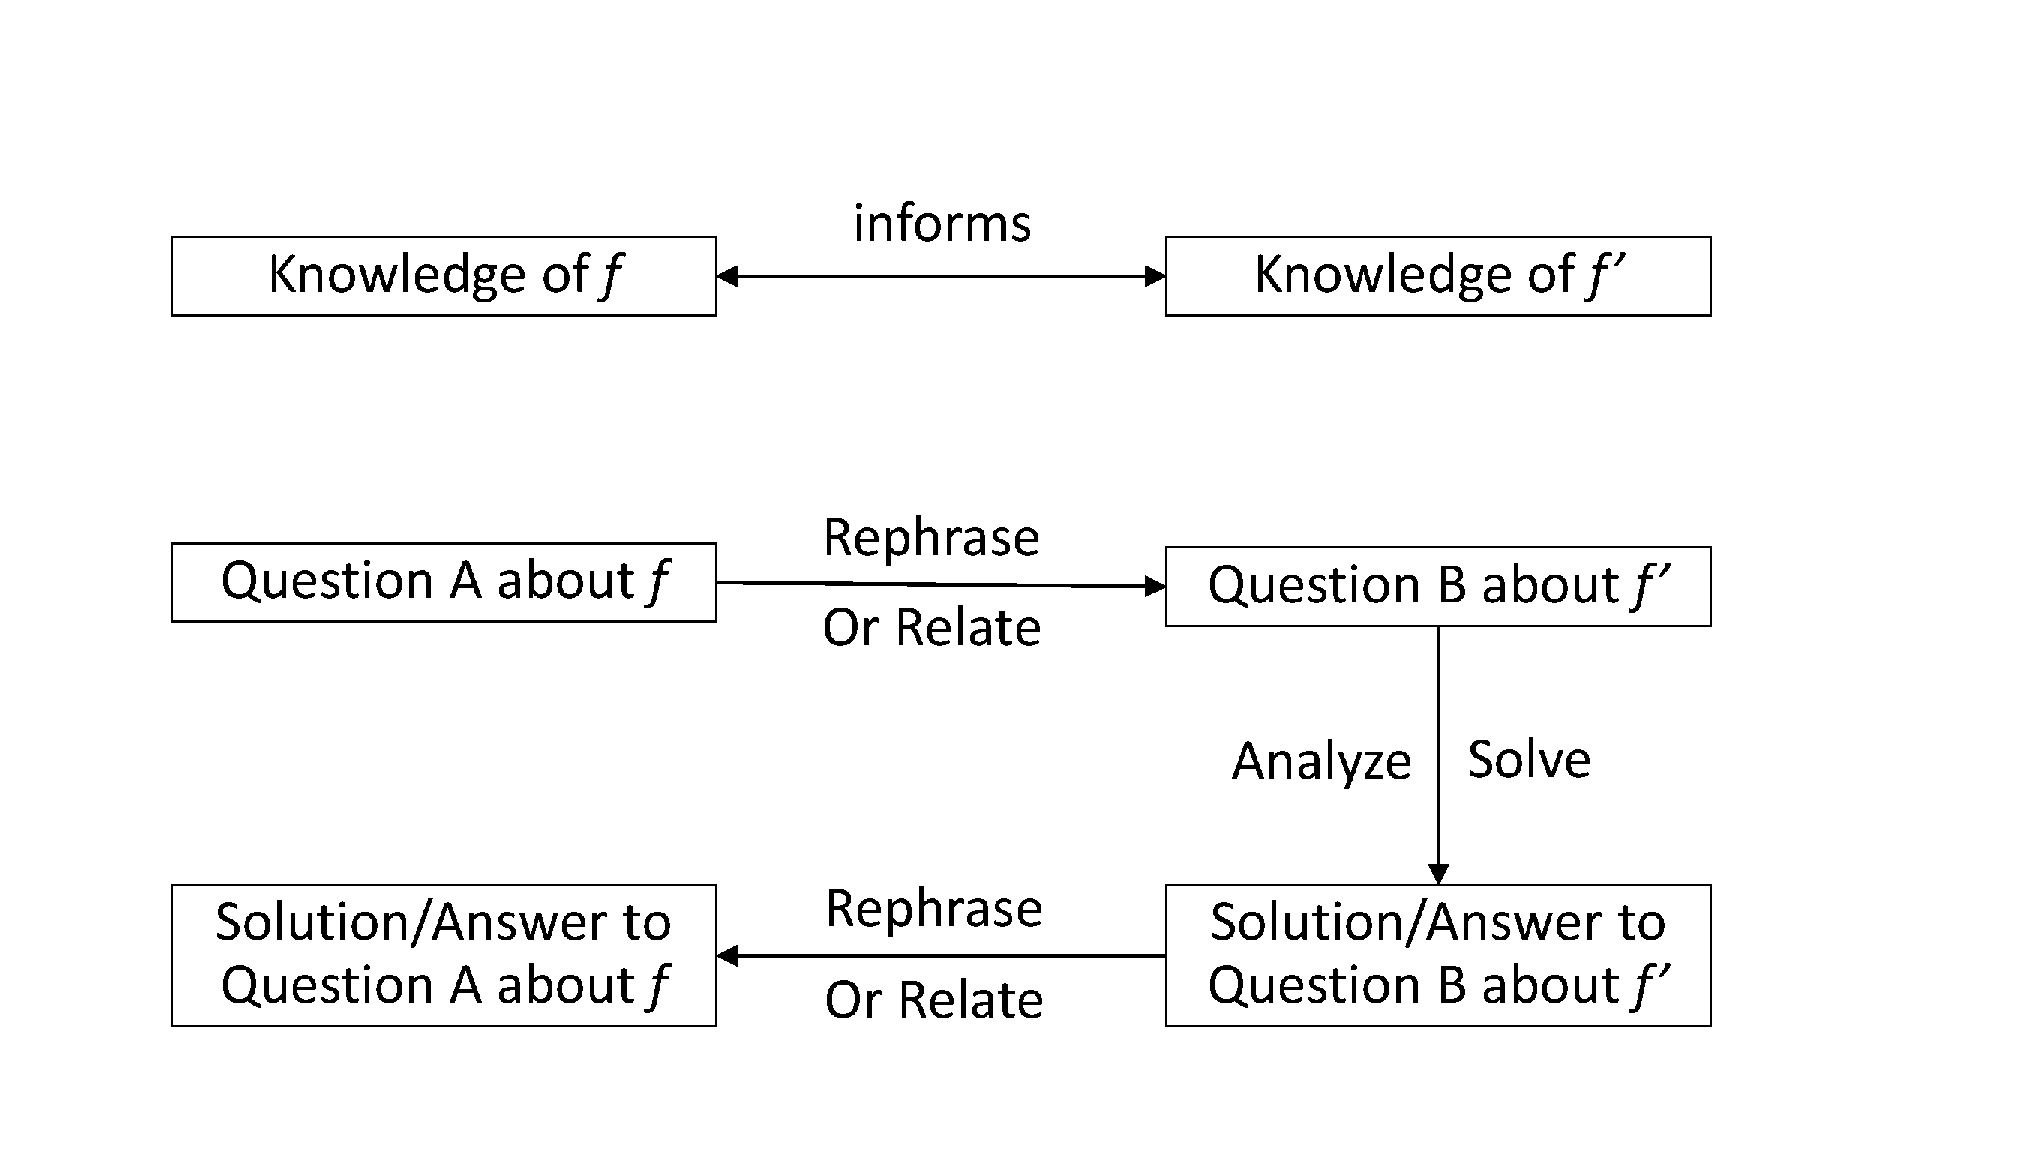
\includegraphics[width=11cm]{images/mvt-intro-diagram-1}$$

The Mean Value Theore tells us that
there is an intimate connection between the net change of the value of any
``sufficiently nice'' function over an
interval and the possible values of its derivative on that interval. Because
of this connection, we can draw conclusions about the possible values of the
derivative based on information about the values of the function, and
conversely, we can draw conclusions about the values of the function based
on information about the values of its derivative.

$$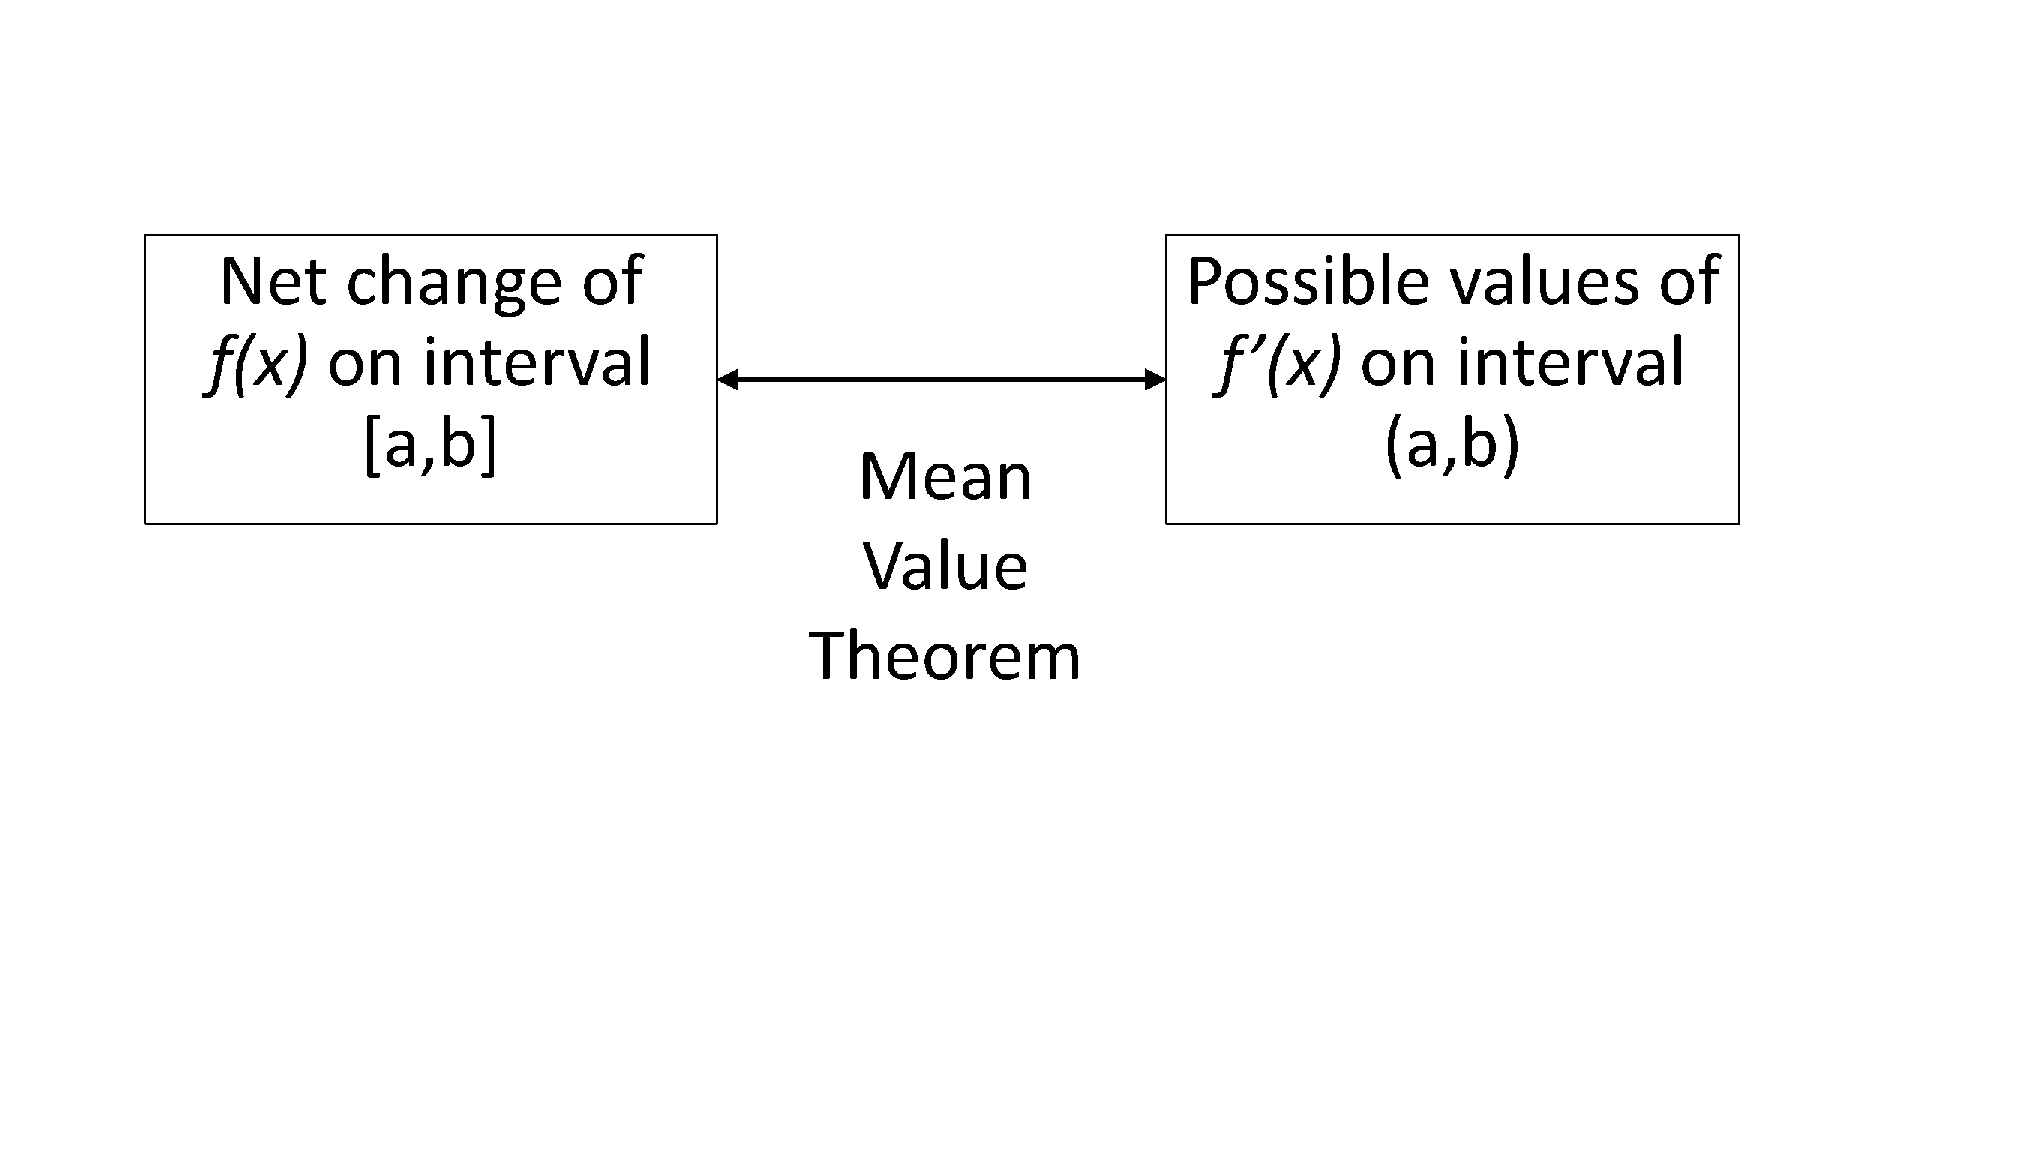
\includegraphics[width=11cm]{images/mvt-intro-diagram-2}$$

Let us illustrate the idea through the following two interesting questions
involving derivatives:

\begin{enumerate}
	\item Suppose two different functions have the same derivative;
		  what can you say about the relationship between the two functions?
	\item Suppose you drive a car from toll booth on a toll road to
		  another toll booth at an average speed of 70 miles per hour. 
		  What can be concluded about your actual speed during the trip? 
		  In particular, did you exceed the 65 mile per hour speed limit?
\end{enumerate}

While these sound very different, it turns out that the two problems
are very closely related. We know that ``speed'' is really the
derivative by a different name; let's start by translating the second
question into something that may be easier to visualize. Suppose that
the function $f(t)$ gives the position of your car on the toll road at
time $t$. Your change in position between one toll booth and the next
is given by $\ds f(t_1)-f(t_0)$, assuming that at time $\ds t_0$ you were at
the first booth and at time $\ds t_1$ you arrived at the second
booth. Your average speed for the trip is
$\ds (f(t_1)-f(t_0))/(t_1-t_0)$. If we think about the graph of $f(t)$,
the average speed is the slope of the line that connects the two
points $\ds (t_0,f(t_0))$ and $\ds (t_1,f(t_1))$. Your speed at any particular time
$t$ between $\ds t_0$ and $\ds t_1$ is $f'(t)$, the slope of the curve. Now
question (2) becomes a question about slope. In particular, if the
slope between endpoints is 70, what can be said of the slopes at
points between the endpoints?

As a general rule, when faced with a new problem it is often a good idea to
examine one or more simplified versions of the problem, in the hope
that this will lead to an understanding of the original problem.
In this case, the problem in its ``slope'' form is somewhat easier to
simplify than the original, but equivalent, problem.
 
Here is a special instance of the problem. Suppose that
$\ds f(t_0)=f(t_1)$. Then the two endpoints have the same height and the
slope of the line connecting the endpoints is zero. What can we say
about the slope between the endpoints? It shouldn't take much
experimentation before you are convinced of the truth of this
statement: Somewhere between $\ds t_0$ and $\ds t_1$ the slope is exactly
zero, that is, somewhere between $\ds t_0$ and $\ds t_1$ the slope is equal to
the slope of the line between the endpoints. This suggests that
perhaps the same is true even if the endpoints are at different
heights, and again a bit of experimentation will probably convince you
that this is so. But we can do better than ``experimentation''---we
can prove that this is so.

We start with the simplified version:

\begin{theorem}{Rolle's Theorem}{rolle}
(Rolle's Theorem) Suppose that $f(x)$ has a derivative on the
interval $(a,b)$, is continuous on the interval $[a,b]$, and
$f(a)=f(b)$. Then at some value $c\in (a,b)$, $f'(c)=0$.
\end{theorem}

\begin{proof}
We know that $f(x)$ has a maximum and minimum value on $[a,b]$
(because it is continuous), and we
also know that the maximum and minimum must occur at an endpoint, at a
point at which the derivative is zero, or at a point where the
derivative is undefined. Since the derivative is never undefined, that
possibility is removed.

If the maximum or minimum occurs at a point $c$, other than an endpoint,
where $f'(c)=0$, then we have found the point we seek. Otherwise, the
maximum and minimum both occur at an endpoint, and since the endpoints
have the same height, the maximum and minimum are the same. This means
that $f(x)=f(a)=f(b)$ at every $x \in [a,b]$, so the function is a
horizontal line, and it has derivative zero everywhere in
$(a,b)$. Then we may choose any $c$ at all to get $f'(c)=0$.
\end{proof}

Rolle's Theorem is illustrated below for a function $f(x)$ where $f'(x)=0$ holds for two values of $x=c_1$ and $x=c_2$:
$$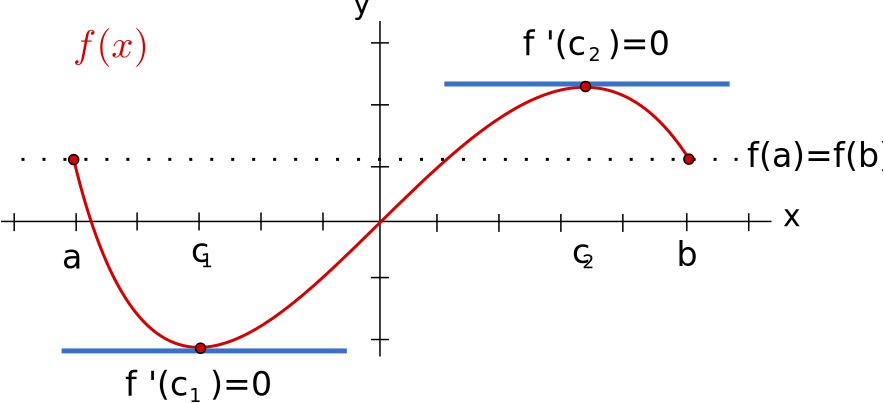
\includegraphics[width=4in]{images/rolle}$$

Perhaps remarkably, this special case is all we need to prove the more
general one as well.

\begin{theorem}{Mean Value Theorem}{mvt} 
Suppose that $f(x)$ has a derivative on the
interval $(a,b)$ and is continuous on the interval $[a,b]$. 
Then at some value $c\in (a,b)$, $\ds f'(c)={f(b)-f(a)\over b-a}$.
\end{theorem}

\begin{proof}
Let $\ds m={f(b)-f(a)\over b-a}$, and consider a new function
$g(x)=f(x) - m(x-a)-f(a)$. We know that $g(x)$ has a derivative
everywhere, since $g'(x)=f'(x)-m$. We can compute 
$g(a)=f(a)- m(a-a)-f(a) =0$ and
\begin{eqnarray*}
g(b)=f(b)-m(b-a)-f(a)&=f(b)-{f(b)-f(a)\over b-a}(b-a)-f(a)\cr
&=f(b)-(f(b)-f(a))-f(a)=0.\cr
\end{eqnarray*}
So the height of $g(x)$ is the same at both endpoints. This means, by
Rolle's Theorem, that at some $c$, $g'(c)=0$. But we know that
$g'(c)=f'(c)-m$, so
$$0=f'(c)-m=f'(c)-{f(b)-f(a)\over b-a},$$
which turns into
$$f'(c)={f(b)-f(a)\over b-a},$$
exactly what we want.
\end{proof}

The Mean Value Theorem is illustrated below showing the existence of a point $x=c$ for a function $f(x)$ where the tangent line at $x=c$ (with slope $f'(c)$) is parallel to the secant line connecting $A(a,f(a))$ and $B(b,f(b))$ (with slope ${f(b)-f(a)\over b-a}$):
$$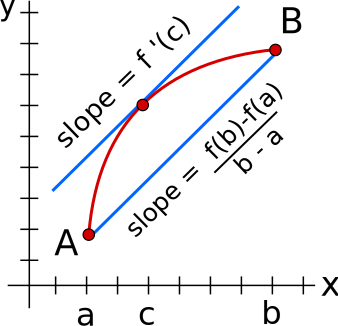
\includegraphics[width=2.0in]{images/mvt}$$

Returning to the original formulation of question (2), we see that if
$f(t)$ gives the position of your car at time $t$, then the Mean Value
Theorem says that at some time $c$, $f'(c)=70$, that is, at some time
you must have been traveling at exactly your average speed for the
trip, and that indeed you exceeded the speed limit.

Now let's return to question (1). Suppose, for example, that two
functions are known to have derivative equal to 5 everywhere,
$f'(x)=g'(x)=5$. It is easy to find such functions: $5x$, $5x+47$,
$5x-132$, etc. Are there other, more complicated, examples? No---the
only functions that work are the ``obvious'' ones, namely, $5x$ plus
some constant. How can we see that this is true?

Although ``5'' is a very simple derivative, let's look at an even
simpler one. Suppose that $f'(x)=g'(x)=0$. Again we can find examples:
$f(x)=0$, $f(x)=47$, $f(x)=-511$ all have $f'(x)=0$. Are there
non-constant functions $f$ with derivative 0? No, and here's why:
Suppose that $f(x)$ is not a constant function. This means that there
are two points on the function with different heights, say
$f(a)\not=f(b)$. The Mean Value Theorem tells us that at some point
$c$, $f'(c)=(f(b)-f(a))/(b-a)\not=0$. So any non-constant function
does not have a derivative that is zero everywhere; this is the same
as saying that the only functions with zero derivative are the
constant functions.

Let's go back to the slightly less easy example: suppose that 
$f'(x)=g'(x)=5$. Then $(f(x)-g(x))' = f'(x)-g'(x) = 5 -5 =0$. So using
what we discovered in the previous paragraph, we know that
$f(x)-g(x)=k$, for some constant $k$. So any two functions with
derivative 5 must differ by a constant; since $5x$ is known to work,
the only other examples must look like $5x+k$.

Now we can extend this to more complicated functions, without any
extra work. Suppose that $f'(x)=g'(x)$. Then as before
$(f(x)-g(x))' = f'(x)-g'(x) =0$, so $f(x)-g(x)=k$. Again this means
that if we find just a single function $g(x)$ with a certain
derivative, then every other function with the same derivative must be
of the form $g(x)+k$.

\begin{example}{Given Derivative}{givenderivative}
Describe all functions that have derivative $5x-3$. 
\end{example}

\begin{solution} 
It's easy to find
one: $\ds g(x)=(5/2)x^2-3x$ has $g'(x)=5x-3$. The only other functions
with the same derivative are therefore of the form
$\ds f(x)=(5/2)x^2-3x+k$.

Alternately, though not obviously, you might have first noticed that 
$\ds g(x)=(5/2)x^2-3x+47$ has $g'(x)=5x-3$. Then every other function
with the same derivative must have the form $\ds f(x)=(5/2)x^2-3x+47+k$.
This looks different, but it really isn't. The functions of the form
$\ds f(x)=(5/2)x^2-3x+k$ are exactly the same as the ones of the form
$\ds f(x)=(5/2)x^2-3x+47+k$. For example, $\ds (5/2)x^2-3x+10$ is the same as
$\ds (5/2)x^2-3x+47+(-37)$, and the first is of the first form while
the second has the second form.
\end{solution}

This is worth calling a theorem:

\begin{theorem}{Functions with the Same Derivative}{FunctionsSameDerivative}
If $f'(x)=g'(x)$ for every $x\in (a,b)$, then for some constant
$k$, $f(x)=g(x)+k$ on the interval $(a,b)$.
\end{theorem} 

\begin{example}{Same Derivative}{SameDerivative}
Describe all functions with derivative $\ds \sin x + e^x$. One such
function is $\ds -\cos x+e^x$, so all such functions have the form
$-\cos x+e^x+k$.
\end{example}

Theorem~\ref{thm:FunctionsSameDerivative} and the above example illustrate what the Mean
Value Theorem allows us to say about $f(x)$ when we have
perfect information about $f^{\prime}(x)$. Specifically, $f(x)$
is determined up to a constant. Our next example
illustrates almost the opposite extreme situation, one where we have much
less information about $f^{\prime}(x)$ beyond the fact that $f^{\prime}(x)$
exists. Specifically, assuming that we know an
upper bound on the values of $f^{\prime}(x)$, what can we say
about the values of $f(x)$?

\begin{example}{Conclusion Regarding Function Value Based on Derivative Information}{FuncValDerivativeInfo}
Suppose that $f$ is a differentiable function such that $f^{\prime }\left(
x\right) \leq 2$ for all $x.$ What is the largest possible value of $f\left(
7\right) $ if $f\left( 3\right) =5?$
\end{example}
\begin{solution}
We are interested in the values of $f\left( x\right) $ at $x=3$
and $x=7.$ It makes sense to focus our attention on the interval between 3
and 7. It is given that $f\left( x\right) $ is differentiable for all $x.$
So, $f\left( x\right) $ is also continuous at all $x.$ In particular, $%
f\left( x\right) $ is continuous on the interval $\left[ 3,7\right] $ and
differentiable on the interval $\left( 3,7\right) .$ By the Mean Value
Theorem, we know that there is some $c$ in $\left( 3,7\right) $ such that 
\begin{equation*}
f^{\prime }\left( c\right) =\frac{f\left( 7\right) -f\left( 3\right) }{7-3}.
\end{equation*}%
Simplifying and using the given information $f\left( 3\right) =5$, we get 
\begin{equation*}
f^{\prime }\left( c\right) =\frac{f\left( 7\right) -5}{4},
\end{equation*}%
or, after re-arranging the terms,%
\begin{equation*}
f\left( 7\right) =4f^{\prime }\left( c\right) +5.
\end{equation*}%
We do not know the exact value of $c,$ but we do know that $f^{\prime
}\left( x\right) \leq 2$ for all $x.$ This implies that $f^{\prime }\left(
c\right) \leq 2.$ Therefore,%
\begin{equation*}
f\left( 7\right) \leq 4\cdot 2+5=13.
\end{equation*}%
That is, the value of $f\left( 7\right) $ cannot exceed 13. To convince
ourselves that 13 (as opposed to some smaller number) is the largest
possible value of $f\left( 7\right) ,$ we still need to show that it is
possible for the value of $f\left( 7\right) $ to reach 13. If we review our
proof, we notice that the inequality will be an equality if $f^{\prime
}\left( c\right) =2.$ One way to guarantee this without knowing anything
about $c$ is to require $f^{\prime }\left( x\right) =2$ for all $x.$ This
means that $f\left( x\right) =2x+k$ for some constant $k.$ From the
condition $f\left( 3\right) =5,$ we see that $k=-1.$ We can easily verify
that indeed $f\left( x\right) =2x-1$ meets all our requirements and $f\left(
7\right) =13$.
\end{solution}


%%%%%%%%%%%%%%%%%%%%%%%%%%%%%%%%%%%%%%%%%%%%%%%%%
\Opensolutionfile{solutions}[ex]
\section*{Exercises for Section \ref{sec:MVT}}

\begin{enumialphparenastyle}

%%%%%%%%%%
\begin{ex}
 Let $\ds f(x) = x^2$.
Find a value $c\in (-1,2)$ so that $f'(c)$ equals the slope between
the endpoints of $f(x)$ on $[-1,2]$.
\begin{sol}
 $c=1/2$
\end{sol}
\end{ex}

%%%%%%%%%%
\begin{ex}
 Verify that $f(x) = x/(x+2)$ satisfies the hypotheses of the
 Mean Value Theorem on the interval $[1,4]$ and then find all of the
 values, $c$, that satisfy the conclusion of the theorem.
\begin{sol}
 $\ds c=\sqrt{18}-2$
\end{sol}
\end{ex}

%%%%%%%%%%
\begin{ex}
Verify that $f(x) = 3x/(x+7)$ satisfies the hypotheses of the
 Mean Value Theorem on the interval $[-2 , 6]$ and then find all of the
 values, $c$, that satisfy the conclusion of the theorem.
\end{ex}

%%%%%%%%%%
\begin{ex}
 Let $f(x) = \tan x $. Show that $f(\pi ) = f(2\pi)=0$ but
there is no number $c\in (\pi,2\pi)$ such that $f'(c) =0$. Why does
this not contradict Rolle's theorem?
\end{ex}

%%%%%%%%%%
\begin{ex}
 Let $\ds f(x) = (x-3)^{-2}$.  Show that there is no value 
$c\in (1,4)$ such that $f'(c) = (f(4)-f(1))/(4-1)$.  Why is
this not a contradiction of the Mean Value Theorem?
\end{ex}

%%%%%%%%%%
\begin{ex}
 Describe all functions with derivative $\ds x^2+47x-5$.
\begin{sol}
 $\ds x^3/3+47x^2/2-5x+k$
\end{sol}
\end{ex}

%%%%%%%%%%
\begin{ex}
 Describe all functions with derivative $\ds {1\over 1+x^2}$.
\begin{sol}
 $\arctan x + k$
\end{sol}
\end{ex}

%%%%%%%%%%
\begin{ex}
 Describe all functions with derivative $\ds x^3-{1\over x}$.
\begin{sol}
 $\ds x^4/4 -\ln x +k$
\end{sol}
\end{ex}

%%%%%%%%%%
\begin{ex}
 Describe all functions with derivative $\sin(2x)$.
\begin{sol}
 $-\cos(2x)/2 +k$
\end{sol}
\end{ex}

\begin{ex}
Find $f\left( x\right) $ if $f^{\prime }\left( x\right) =e^{-x}$ and $%
f\left( 0\right) =2$.
\end{ex}

\begin{ex}
Suppose that $f$ is a differentiable function such that $f^{\prime }\left(
x\right) \geq -3$ for all $x.$ What is the smallest possible value of $%
f\left( 4\right) $ if $f\left( -1\right) =2$?
\end{ex}

%%%%%%%%%%
\begin{ex}
 Show that the equation $\ds 6x^4 -7x+1 =0$ does not have more
than two distinct real roots.
\end{ex}

%%%%%%%%%%
\begin{ex}
 Let $f$ be differentiable on $\R$. Suppose that $f'(x) \neq
0$ for every $x$. Prove that $f$ has at most one real root.
\end{ex}
 
%%%%%%%%%%
\begin{ex}
 Prove that for all real $x$ and $y$
$|\cos x -\cos y | \leq |x-y|$.
State and prove an analogous result involving sine.
\end{ex}

%%%%%%%%%%
\begin{ex}
Show that $\ds \sqrt{1+x} \le 1 +(x/2)$ if $-1<x<1$.
\end{ex}

%%%%%%%%%%
\begin{ex}
Suppose that $f(a)=g(a)$
and that $f^{\prime}(x)\leq g^{\prime}(x)$ for
all $x\geq a$.
\begin{enumerate}
	\item	Prove that $f(x)\leq g(x)$ for all $x\geq a$.
	\item	Use part (a) to prove that $e^x\geq 1+x$ for all $x\geq	0$.
	\item	Use parts (a) and (b) to prove that $e^x\geq 1+x+\dfrac{x^2}{2}$ for all $x\geq 0$.
	\item	Can you generalize these results?
\end{enumerate}
\end{ex}

\end{enumialphparenastyle}
